% Section-local compatibility helpers; packages are loaded by main.tex.
\providecommand{\tightlist}{%
  \setlength{\itemsep}{0pt}\setlength{\parskip}{0pt}}
\providecommand{\maxwidth}{\linewidth}
\providecommand{\maxheight}{\textheight}



\section{User Interface and User Experience Design}\label{user-interface-and-user-experience-design}

This section describes the proposed user interface and user experience
design of Room4U. It defines the screen structure, navigation flows,
detailed screen specifications, control behaviors, validation rules,
event handling, error feedback, responsive layout, and accessibility
considerations.

The design follows the eight screen identifiers (S01--S08) and the
Student and Administrator interfaces established in PA2. The PA2 mockups
are reused as the visual basis for the corresponding PA3 screens. The
control specifications below clarify how the proposed interface should
behave during implementation and verification.

\subsection{Screen List and Flow}\label{screen-list-and-flow}

\subsubsection{7.1.1. Screen List}\label{screen-list}

Room4U provides two role-based interfaces. The Student Interface
supports room discovery, booking requests, request tracking, and
history. The Administrator Interface supports request processing, room
management, and maintenance management.

\small
\setlength{\tabcolsep}{3pt}
\renewcommand{\arraystretch}{1.15}
\begin{longtable}[]{@{}
  >{\raggedright\arraybackslash}p{0.10\textwidth}
  >{\raggedright\arraybackslash}p{0.205\textwidth}
  >{\raggedright\arraybackslash}p{0.16\textwidth}
  >{\raggedright\arraybackslash}p{0.455\textwidth}@{}}
\hline
\begin{minipage}[b]{\linewidth}\raggedright
\textbf{ID}
\end{minipage} & \begin{minipage}[b]{\linewidth}\raggedright
\textbf{Screen Name}
\end{minipage} & \begin{minipage}[b]{\linewidth}\raggedright
\textbf{Use Cases}
\end{minipage} & \begin{minipage}[b]{\linewidth}\raggedright
\textbf{Purpose}
\end{minipage} \\
\hline
\endhead
\hline
\endlastfoot
\textbf{S01} & Sign In & UC-01 & Entry point for Student and
Administrator authentication using provided accounts. \\
\textbf{S02} & Room Search and Availability & UC-02, UC-03 & Search for
suitable rooms and inspect their schedules before requesting a
booking. \\
\textbf{S03} & Booking Request & UC-04 & Submit a booking request for a
selected room using date, start time, duration, group size, purpose, and
optional note. \\
\textbf{S04} & My Requests and History & UC-02, UC-05, UC-06 & Monitor
submitted requests, inspect request details, cancel eligible requests,
and review processed requests. \\
\textbf{S05} & Admin Request Queue & UC-02, UC-07 & Review, search, and
filter student booking requests. \\
\textbf{S06} & Booking Request Details and Processing & UC-07, UC-08,
UC-09, UC-10 & Inspect request details and process Pending or Approved
requests when permitted. \\
\textbf{S07} & Room Management & UC-11, UC-12 & Add and update room
records and suspend or resume rooms. \\
\textbf{S08} & Room Availability and Maintenance & UC-13 & Inspect room
usage and manage maintenance schedules. \\
\end{longtable}
\normalsize

\subsubsection{7.1.2. Navigation Flow}\label{navigation-flow}

\textbf{Student Navigation Flow}

\begin{enumerate}
\def\labelenumi{\arabic{enumi}.}
\item
  Students open S01 and sign in using an account provided by the system.
\item
  After successful authentication, the application verifies the
  user's role and opens S02 for a Student.
\item
  Students search for rooms using the intended date, number of people,
  and room requirements. They can inspect room details and availability.
\item
  After selecting a room and a suitable time slot, students open S03 to
  complete the booking request.
\item
  After a booking request is submitted, the system returns the
  request's actual status and request ID. S04 displays
  the returned request information; the interface must not assume that
  every submission is Pending.
\item
  Students can open S04 directly from the Student navigation menu at any
  time, including before submitting a new request. From S04, they can
  monitor their requests, inspect full request details, cancel an
  eligible request, and review previously processed requests in History.
\item
  Students can open S02 from the Student navigation menu to search for
  rooms, open S03 from a selected room and time slot to submit a booking
  request, or open S04 directly from the menu. They can use Log Out to
  return to S01.
\end{enumerate}

\textbf{Administrator Navigation Flow}

\begin{enumerate}
\def\labelenumi{\arabic{enumi}.}
\item
  Administrators open S01 and sign in using an account provided by the
  system.
\item
  After successful authentication, the application verifies the
  user's role and opens the Administrator interface.
  S05, S07, and S08 are each directly accessible from the Administrator
  navigation menu.
\item
  Administrators can open S05 directly from the menu to review the
  request queue and filter requests by Pending, Approved, Rejected, or
  Cancelled status.
\item
  Selecting View Details from S05 opens S06. From S06, the administrator
  can inspect the selected request, perform permitted approval,
  rejection, or cancellation actions, and return to S05.
\item
  Administrators can open S07 directly from the navigation menu to add
  rooms, edit room information, and suspend or resume rooms.
\item
  Administrators can open S08 directly from the navigation menu to
  inspect room usage, view maintenance schedules, create maintenance
  blocks, and remove eligible future maintenance blocks.
\end{enumerate}

\textbf{Common Navigation and Session Handling}

The Sign In screen is shared by both roles. The application must verify
authentication and the assigned role before opening protected screens.
Student users must not access administrator-only screens or actions.
Administrator users must not submit student booking requests.

The Log Out option is available from the navigation area. Selecting it
opens a confirmation dialog with Cancel and Log Out actions. Cancel
closes the dialog and keeps the user on the current screen. Log Out ends
the session and returns the user to S01. The PA3 design additionally
requires clearing private client-side data and preventing browser
navigation from restoring a protected view after sign-out.

\emph{Figure~\ref{fig:role-based-navigation-flow} shows the main role-based navigation paths. S02 leads
to S03 when a student selects a room and time slot; S04 is independently
accessible from the Student menu. S05 and S06 provide queue-to-detail
and return navigation, while S05, S07, and S08 are independently
accessible from the Administrator menu. Screen transitions remain
subject to authentication, authorization, request status, and the
relevant booking or maintenance rules.}

\begingroup
\renewcommand{\thefigure}{7.1.2}
\refstepcounter{figure}
\label{fig:role-based-navigation-flow}
\begin{center}
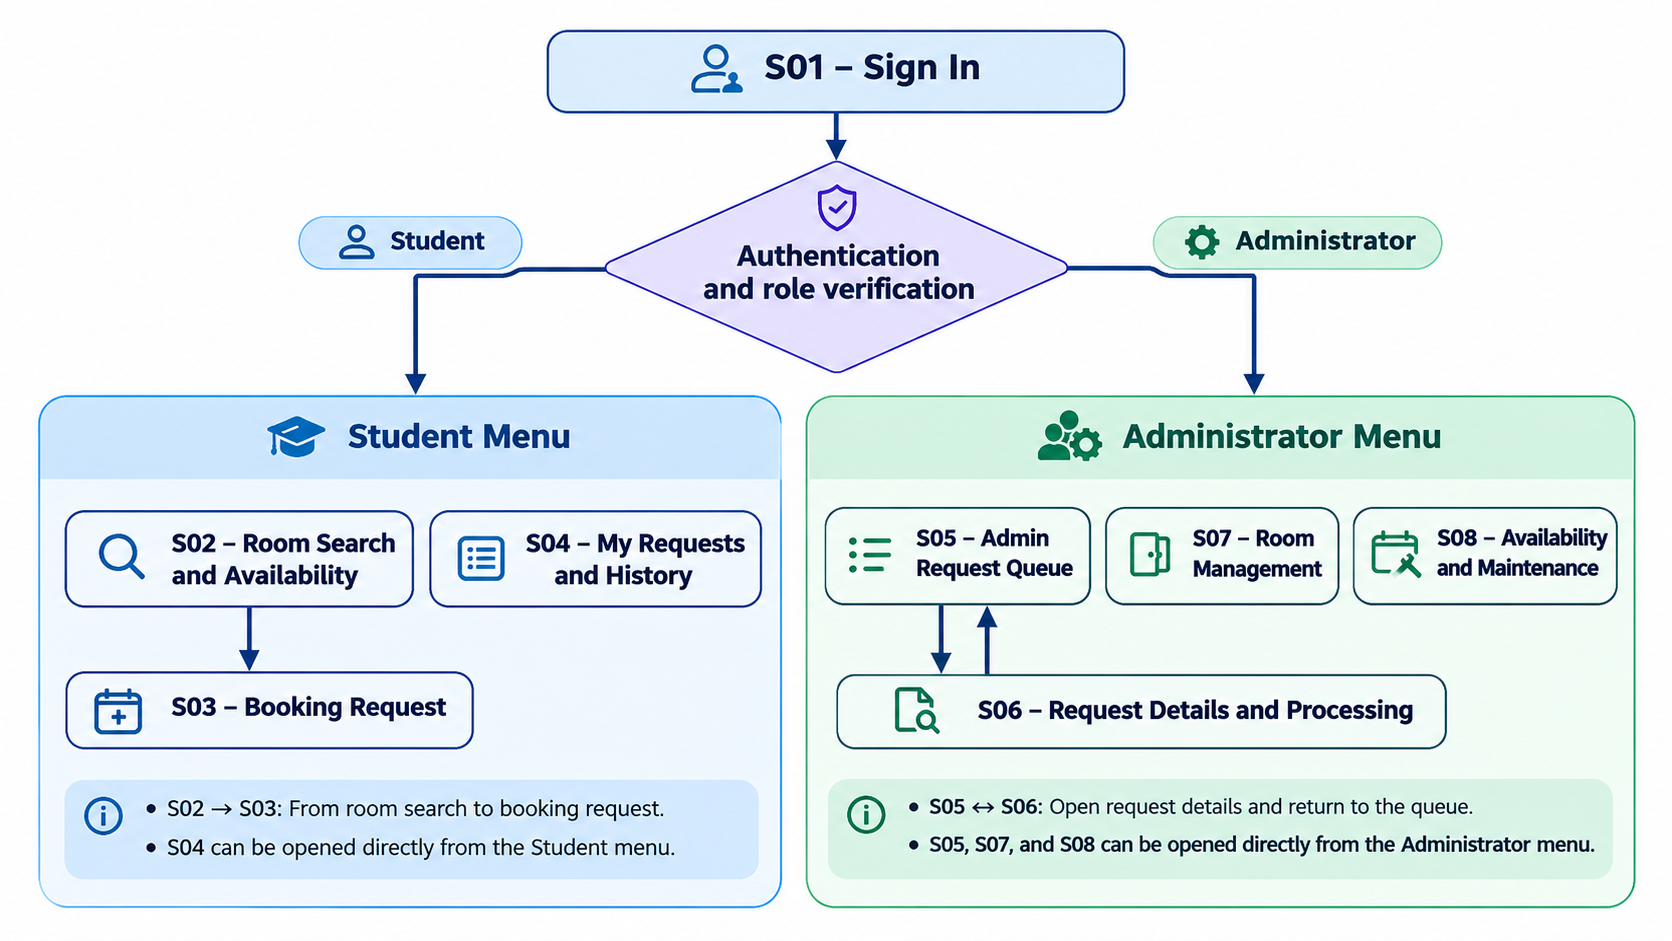
\includegraphics[width=\textwidth,height=0.72\textheight,keepaspectratio]{images/figures/image1.png}
\emph{\textbf{Figure \thefigure.} Proposed role-based navigation flow.}
\end{center}
\endgroup


\subsection{Screen Designs and Detailed
Specifications}\label{screen-designs-and-detailed-specifications}

The following subsections describe the eight screens using the
corresponding mockups from PA2. Detailed control specifications are
provided for S02, S03, S04, S06, S07, and S08. The interface labels
shown in the mockups are Vietnamese, consistent with the Room4U target
users.

\subsubsection{7.2.1. S01 -- Sign In}\label{s01-sign-in}

\textbf{Description:} This screen is the entry point for both Student
and Administrator users. It provides Email and Password fields and a
Sign In button. Users sign in with accounts provided by the system; no
public registration flow is shown. The screen includes Room4U branding
and a short explanation of the service. If authentication fails, an
error message is displayed so the user can check the credentials and try
again.

\textbf{Interaction and Error Handling:} Successful authentication is
followed by application-role verification and navigation to the
appropriate role-based home screen. Failed authentication displays a
generic credential error and allows the user to retry. Registration and
password recovery are outside the PA2 scope.

\begin{center}
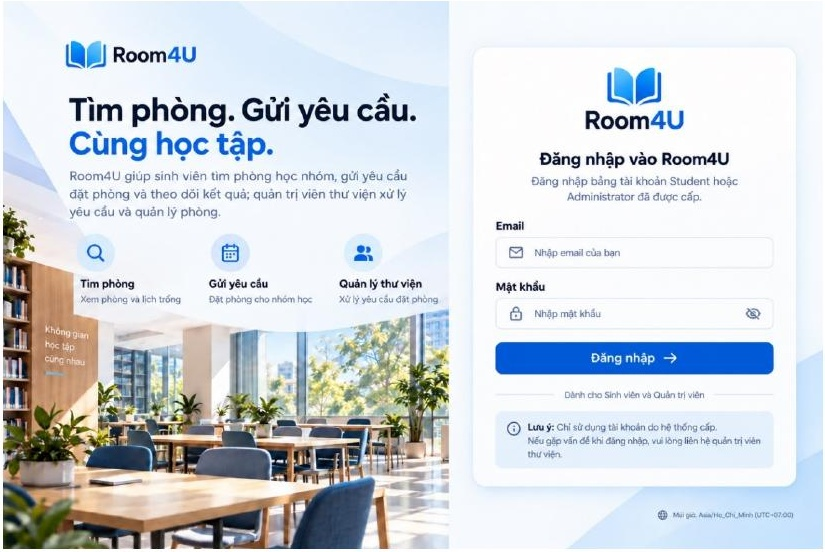
\includegraphics[width=\textwidth,height=0.72\textheight,keepaspectratio]{images/figures/image2.jpg}
\emph{\textbf{Figure 7.2.1.} S01 -- Sign In.}
\end{center}


\subsubsection{7.2.2. S02 -- Room Search and
Availability}\label{s02-room-search-and-availability}

\textbf{Description:} This flow helps students find a suitable meeting
room and check its schedule before submitting a booking request. It
consists of room-search results and a room-availability view.

Room Search: Students can search using the intended date, number of
people, and room requirements. Equipment filters use the equipmentCodes
catalogue defined in ADR-005. Multiple selected equipment codes are
combined using AND logic: a room is returned only when it has every
selected equipment item. Results are presented as room cards showing a
room image, room name, capacity, floor, equipment, current status, and
an action to inspect the room or its availability.

\textbf{Room Availability:} After selecting a room, students can view
its time-slot schedule for a selected date. The schedule distinguishes
available periods from approved bookings, maintenance periods, and other
unavailable periods so that students can choose a valid time before
opening the booking-request form.

\textbf{Control Specifications}

\small
\setlength{\tabcolsep}{3pt}
\renewcommand{\arraystretch}{1.15}
\begin{longtable}[]{@{}
  >{\raggedright\arraybackslash}p{0.15557200000000002\textwidth}
  >{\raggedright\arraybackslash}p{0.15557200000000002\textwidth}
  >{\raggedright\arraybackslash}p{0.317952\textwidth}
  >{\raggedright\arraybackslash}p{0.290904\textwidth}@{}}
\hline
\begin{minipage}[b]{\linewidth}\raggedright
\textbf{Control}
\end{minipage} & \begin{minipage}[b]{\linewidth}\raggedright
\textbf{Type}
\end{minipage} & \begin{minipage}[b]{\linewidth}\raggedright
\textbf{Description and Validation}
\end{minipage} & \begin{minipage}[b]{\linewidth}\raggedright
\textbf{Event Handling}
\end{minipage} \\
\hline
\endhead
\hline
\endlastfoot
\textbf{Date filter} & Date input & Selects the intended booking date;
must be a valid date. & Search refreshes room results and the
availability view for the selected date. \\
\textbf{Number of people} & Number input / filter & Used to filter rooms
by capacity. & Applying the filter updates the displayed room cards. \\
\textbf{Room requirements} & Checkbox filters & Filters rooms by the
selected equipmentCodes from the ADR-005 equipment catalogue. When
multiple codes are selected, AND logic applies: the room must contain
all selected equipment. An empty selection applies no equipment
restriction. & Changing equipment selections refreshes the search
results using the selected equipmentCodes. \\
\textbf{Room card} & Selectable card & Shows room image, name, capacity,
floor, equipment, and current status. & Selecting the card or
availability action opens the room-availability view. \\
\textbf{Availability schedule} & Calendar / time-slot view &
Distinguishes available, approved-booking, maintenance, and other
unavailable periods. & Selecting a valid time proceeds to the
booking-request form. \\
\end{longtable}
\normalsize

\textbf{Event and Error Handling:} If room-search criteria are invalid,
the interface should identify the relevant input. If room or schedule
data cannot be loaded, the system should display an error and allow
retry. A failed schedule load must not be represented as an empty/free
schedule. Pending requests do not reserve room capacity; availability is
determined by the applicable approved-booking and maintenance records.

\begin{center}
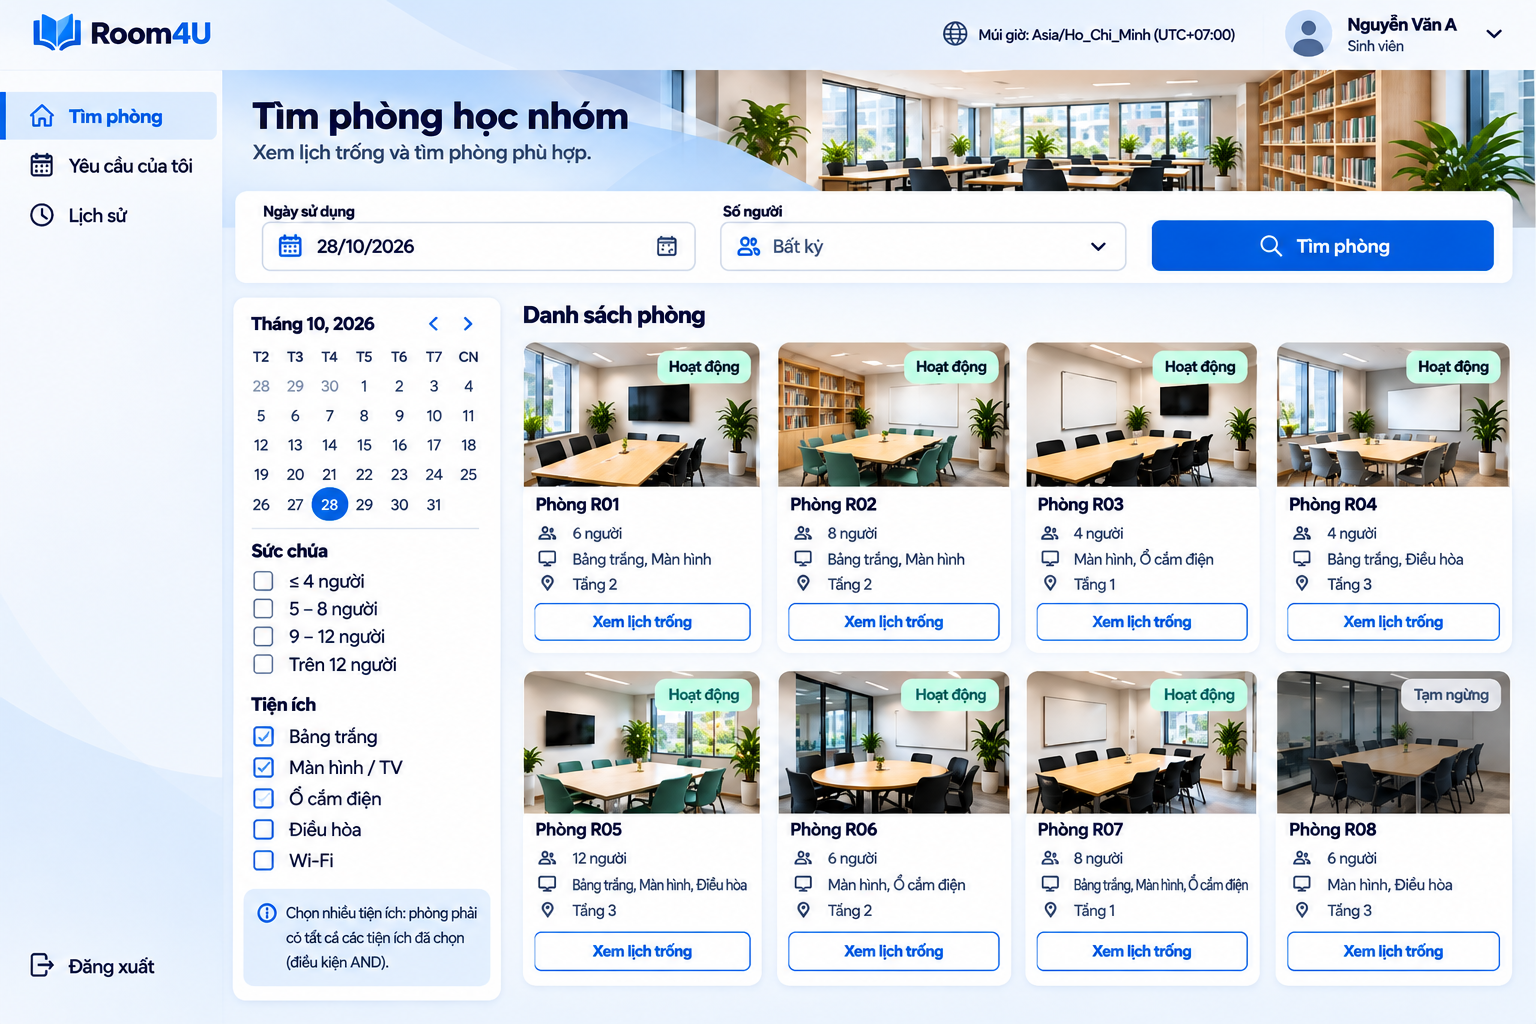
\includegraphics[width=\textwidth,height=0.72\textheight,keepaspectratio]{images/figures/image3.png}
\emph{\textbf{Figure 7.2.2.1.} S02.1 -- Room Search.}
\end{center}


\begin{center}
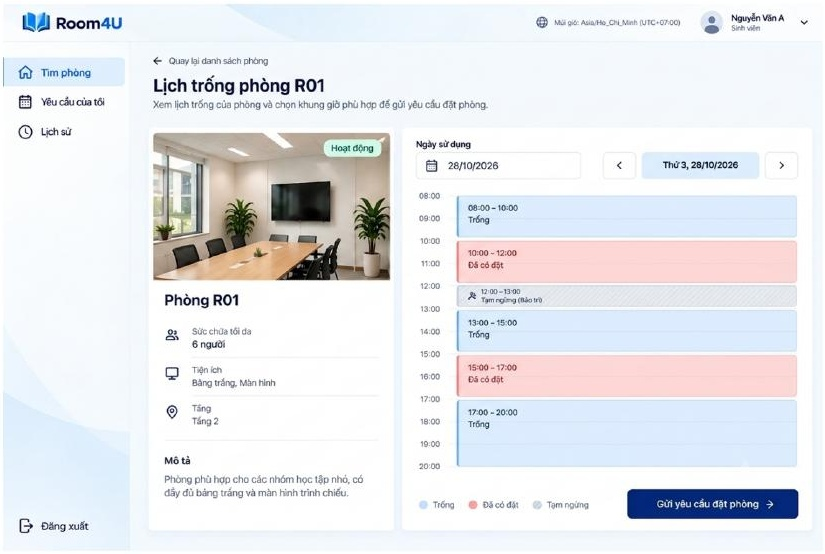
\includegraphics[width=\textwidth,height=0.72\textheight,keepaspectratio]{images/figures/image4.jpg}
\emph{\textbf{Figure 7.2.2.2.} S02.2 -- Room Availability.}
\end{center}


\subsubsection{7.2.3. S03 -- Booking Request}\label{s03-booking-request}

Description: This screen allows a student to submit a booking request
for the selected room. The form displays the room information and
collects the usage date, start time, duration, number of participants,
purpose of use, and an optional note. Purpose of use is a required
dropdown containing only the five purpose codes and Vietnamese labels
defined in ADR-005; arbitrary free text is not accepted. The selected
purpose code is submitted in the purpose API field. The available
duration options are 30, 60, 90, and 120 minutes. Start times must
follow 30-minute increments. The system calculates the end time from the
selected start time and duration. The entire booking must fall within
08:00--20:00 on the same calendar day. The start time must be later than
the current time and no more than seven days from the current time
(BR-04). The participant count must be an integer from 1 through the
selected room's current capacity. The optional note is
limited to 250 characters. The system validates the request against room
capacity, availability, and applicable booking rules.

\textbf{Control Specifications}

\small
\setlength{\tabcolsep}{3pt}
\renewcommand{\arraystretch}{1.15}
\begin{longtable}[]{@{}
  >{\raggedright\arraybackslash}p{0.15557200000000002\textwidth}
  >{\raggedright\arraybackslash}p{0.14885600000000002\textwidth}
  >{\raggedright\arraybackslash}p{0.33147600000000005\textwidth}
  >{\raggedright\arraybackslash}p{0.284096\textwidth}@{}}
\hline
\begin{minipage}[b]{\linewidth}\raggedright
\textbf{Control}
\end{minipage} & \begin{minipage}[b]{\linewidth}\raggedright
\textbf{Type}
\end{minipage} & \begin{minipage}[b]{\linewidth}\raggedright
\textbf{Description and Validation}
\end{minipage} & \begin{minipage}[b]{\linewidth}\raggedright
\textbf{Event Handling}
\end{minipage} \\
\hline
\endhead
\hline
\endlastfoot
\textbf{Selected room} & Read-only summary & Displays selected room
information and current capacity. & Change room returns to S02; no
request is submitted. \\
\textbf{Usage date and start time} & Date/time input & Start time must
be later than the current time, no more than seven days ahead (BR-04),
and aligned to a 30-minute increment. The complete booking interval must
remain within 08:00--20:00 on the same calendar day. & Client-side
validation assists the user; server performs authoritative validation at
submission. \\
\textbf{Duration} & Selection control & Only 30, 60, 90, and 120 minutes
are available. The calculated end time must not exceed 20:00 or cross
into another calendar day. & System calculates and displays the end
time; no independent end-time input is introduced. \\
\textbf{Number of participants} & Number input & Required integer from 1
through the selected room's current capacity. & Invalid
value displays field-level feedback. \\
\textbf{Purpose of use} & Required dropdown & Required selection from
the five values defined in ADR-005. The UI displays the corresponding
Vietnamese label and does not accept arbitrary text. The selected value
is submitted in the purpose API field. & The selected purpose value is
included in the submitted request under the purpose API field. \\
\textbf{Optional note} & Text area & Optional text area; maximum 250
characters. The value is stored in the note field. & The note value is
submitted as note; an empty value means no note was provided. \\
\textbf{Submit / confirmation} & Button and dialog & Student reviews the
booking information before submission. A submissionKey identifies the
logical submission and is retained when retrying the same unchanged
submission after an uncertain response or timeout. & On retry with
unchanged data, the frontend reuses the same submissionKey. If the API
reports that the request already exists, the UI displays that existing
request's actual status and details; it must not create
a duplicate or assume Pending. \\
\end{longtable}
\normalsize

Error Handling and Submission Retry: The system identifies missing or
invalid input and allows the student to correct it. If the room is no
longer available or another booking conflict exists, the request is not
accepted and the interface explains the conflict. A success message is
displayed only after the API confirms the result. If the response is
lost or times out and the outcome is uncertain, retrying the same
unchanged submission must reuse the original submissionKey; a timeout
alone must not cause the frontend to generate a new key. If the API
reports that a request with that key already exists, the interface
displays the existing request and its actual current status returned by
the API. It must not create another request or default the status to
Pending.

\begin{center}
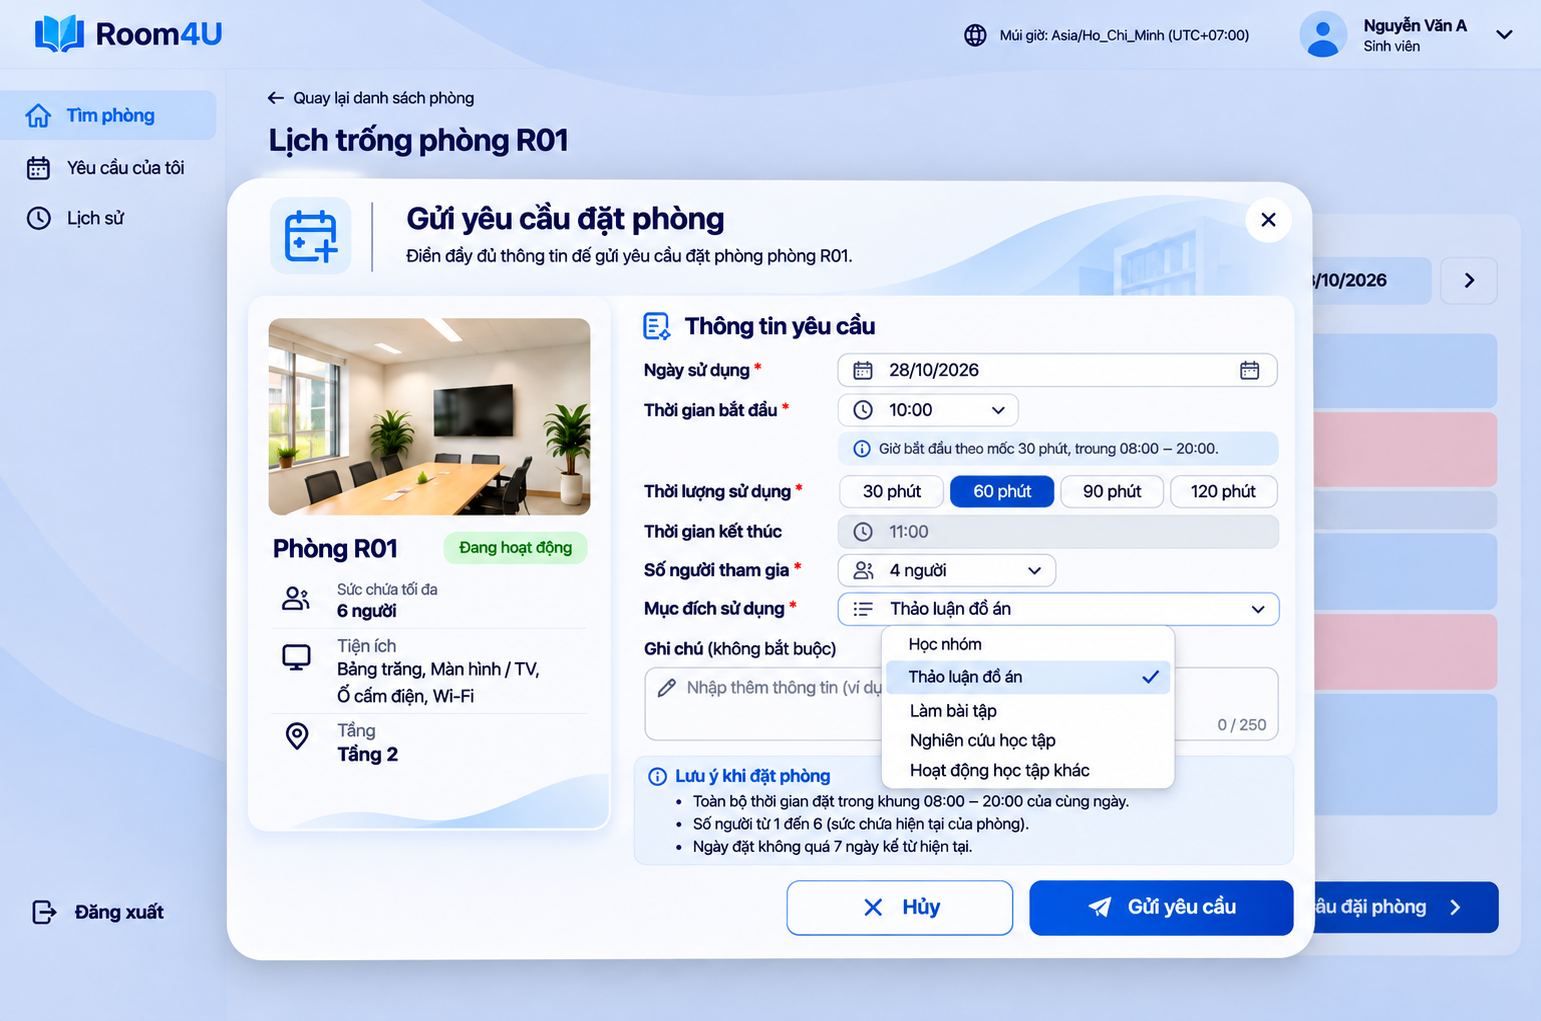
\includegraphics[width=\textwidth,height=0.72\textheight,keepaspectratio]{images/figures/image5.png}
\emph{\textbf{Figure 7.2.3.1.} S03 -- Booking Request form.}
\end{center}


\begin{center}
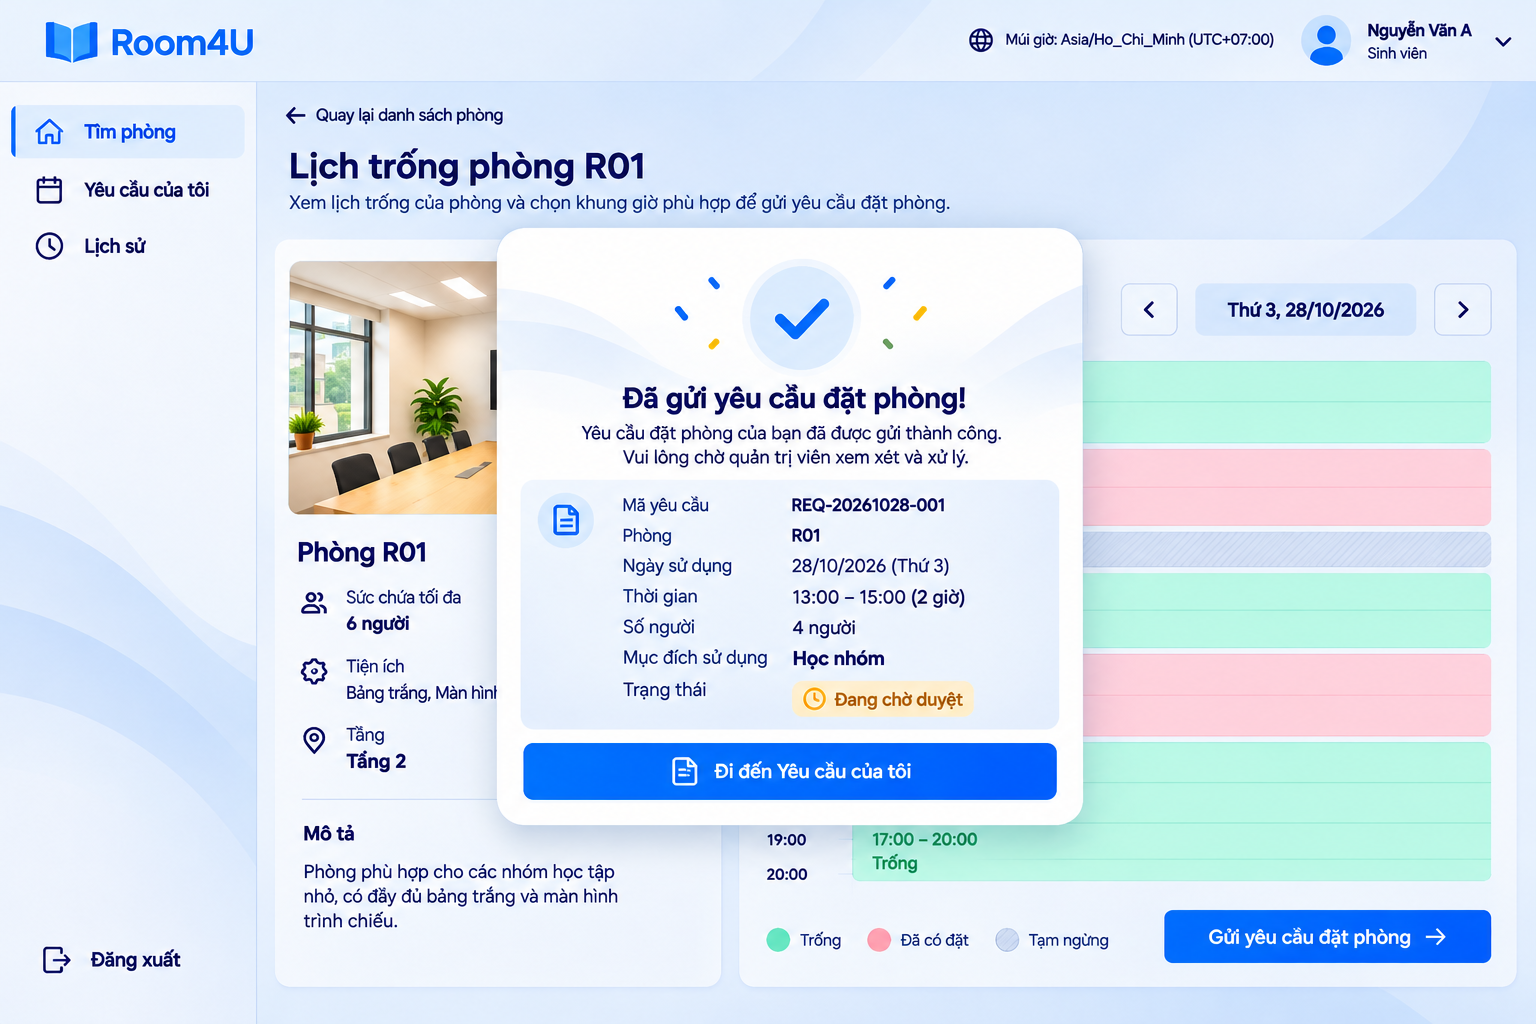
\includegraphics[width=\textwidth,height=0.72\textheight,keepaspectratio]{images/figures/image6.png}
\emph{Figure 7.2.3.2. S03 -- Successful Booking Request Submission.}
\end{center}


\subsubsection{7.2.4. S04 -- My Requests and
History}\label{s04-my-requests-and-history}

\textbf{Description:} This area allows students to monitor submitted
booking requests and review requests that have already been processed.
The active-request screen provides search and status filters. Each row
shows the request ID, room, usage date and time, purpose, current
status, and a View Details action. Students can open a request to
inspect its full information. A separate History screen lists previously
processed requests.

\subsubsection{S04.1 -- My Requests List}\label{s04.1-my-requests-list}

This screen displays the student's request list. Status
tabs help students narrow the results, while the search field supports
searching by request ID, room, or purpose. The table presents the
request ID, room, usage date and time, purpose, status, and a View
Details action. Pagination is provided when the results exceed one page.

\begin{center}
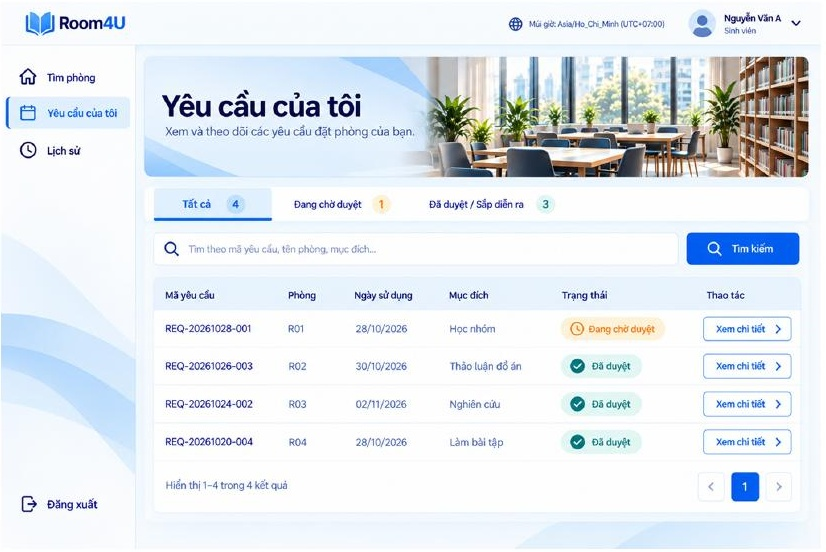
\includegraphics[width=\textwidth,height=0.72\textheight,keepaspectratio]{images/figures/image7.jpg}
\emph{\textbf{Figure 7.2.4.1.} S04.1 -- My Requests List.}
\end{center}


\subsubsection{S04.2 -- Booking Request Details
(Revised)}\label{s04.2-booking-request-details-revised}

This screen presents the full information for one selected request. It
includes the request ID and current status, requester information, room
information, booking information, purpose, and the optional note. The
section labeled ``Mô tả chi tiết yêu
cầu'' displays the content of the note field; it is not
a separate data field.

\begin{itemize}
\item
  \textbf{Requester Information:} Full name, student ID, email address,
  and phone number. These values are supplied from the database.
\item
  \textbf{Room Information:} Room code, room name, building, floor,
  capacity, and equipment. The building information is retained as
  ``Thư viện'' and the floor is retained
  as ``Tầng: 2''. No separate
  room-area/location line is displayed.
\item
  \textbf{Booking Information:} Exactly three evenly arranged
  information cards: ``Thời gian sử dụng'',
  ``Số người đặt'', and
  ``Mục đích sử dụng''.
\item
  Request Description: The purpose is displayed using the Vietnamese
  label mapped from the code stored in the purpose field returned by the
  API. The section labeled ``Mô tả chi tiết yêu
  cầu'' displays the note value. No separate
  detailed-description field exists. Students may mention a course name
  in the optional note; Room4U does not manage enrolled subjects.
\item
  Equipment Information: Equipment labels are resolved from the
  equipment codes returned by the API and displayed using the Vietnamese
  labels in ADR-005.
\item
  \textbf{Request Actions:} Cancel Request is available when the
  applicable request-status and booking-time conditions permit
  cancellation.
\end{itemize}

The ``Môn học liên quan'' field, its book
icon, and its sample value are removed. The ``Vị trí:
Tầng 2, khu A'' line and its location icon are removed.
Room codes such as A-01 and B-01 remain because they are room
identifiers, not area-management data.

\textbf{Control Specifications}

\small
\setlength{\tabcolsep}{3pt}
\renewcommand{\arraystretch}{1.15}
\begin{longtable}[]{@{}
  >{\raggedright\arraybackslash}p{0.15557200000000002\textwidth}
  >{\raggedright\arraybackslash}p{0.14885600000000002\textwidth}
  >{\raggedright\arraybackslash}p{0.33147600000000005\textwidth}
  >{\raggedright\arraybackslash}p{0.284096\textwidth}@{}}
\hline
\begin{minipage}[b]{\linewidth}\raggedright
\textbf{Control}
\end{minipage} & \begin{minipage}[b]{\linewidth}\raggedright
\textbf{Type}
\end{minipage} & \begin{minipage}[b]{\linewidth}\raggedright
\textbf{Description and Validation}
\end{minipage} & \begin{minipage}[b]{\linewidth}\raggedright
\textbf{Event Handling}
\end{minipage} \\
\hline
\endhead
\hline
\endlastfoot
\textbf{Owned request list} & List / compact table & Displays only the
authenticated student's requests and their textual
statuses. & Select opens the corresponding owned request detail; empty
state offers navigation to S02. \\
\textbf{Search} & Text input & Supports request ID, room, or purpose. &
Updates the displayed request list. \\
\textbf{Status filters} & Tabs / selection control & Filters by the
statuses shown in the PA2/PA3 design. & Selecting a status updates the
list without changing request records. \\
\textbf{Request details} & Read-only information & Shows request
ID/status; requester name, student ID, email, phone; room code/name,
building, floor, capacity, equipment; usage period, participant count,
purpose label resolved from the code stored in the purpose API field,
and the note displayed as ``Mô tả chi tiết yêu
cầu''. The note is not a separate field. No subject or
room-area field. & Selecting a request opens details; refresh retrieves
current information. \\
\textbf{Processing history} & Read-only event list & Shows request
events, actor/time, and applicable processing or cancellation reason. &
Refresh retrieves the current request state and history. \\
\textbf{Cancel Request} & Button + confirmation & Only for the
student's own eligible Pending or Approved request
before the scheduled start time. & Confirmation invokes UC-06;
cancel/close leaves the request unchanged. \\
\textbf{Conflict / load feedback} & Status message / retry & Must not
assume cancellation succeeded if the response is lost or uncertain. &
Refresh retrieves the actual request state before displaying the
result. \\
\end{longtable}
\normalsize

\textbf{Cancellation Interaction:} When a student selects Cancel Request
for an eligible request, the system asks for confirmation before
changing the request status. If cancellation is not allowed, the
interface explains why the action cannot proceed. Closing the dialog or
choosing not to continue leaves the request unchanged.

\textbf{History Function:} The History screen allows students to review
previously processed booking requests. It includes Rejected and
Cancelled requests, as well as Approved requests whose scheduled usage
time has passed. An Approved request retains its Approved status; the
interface may indicate that its scheduled time has passed rather than
changing the status to Completed. The history table shows the request
ID, room, usage date, purpose, status, and a View Details action. Search
and pagination help students locate older records.

\textbf{Logout Interaction:} The Log Out option is available in the left
navigation. Selecting it opens a confirmation dialog. Cancel closes the
dialog and keeps the student on the current page; Log Out ends the
session and returns the user to S01.

\begin{center}
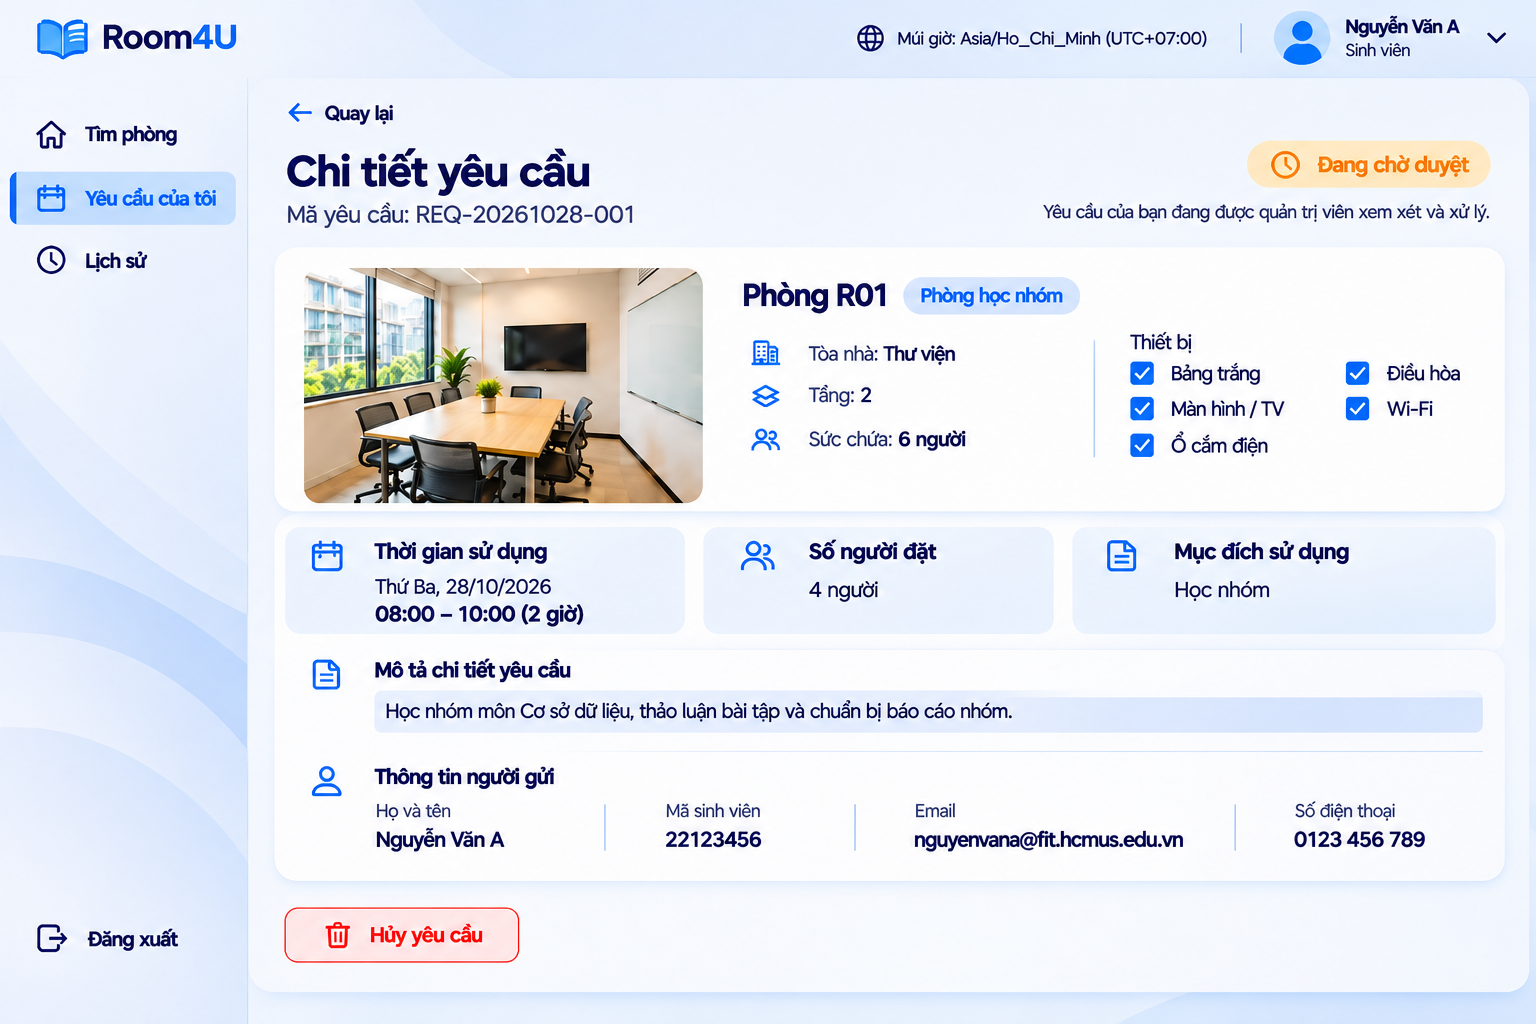
\includegraphics[width=\textwidth,height=0.72\textheight,keepaspectratio]{images/figures/image8.png}
\emph{\textbf{Figure 7.2.4.2.} S04.2 -- Booking Request Details (PA2 mockup
revised to remove subject and room-area fields).}
\end{center}


\begin{center}
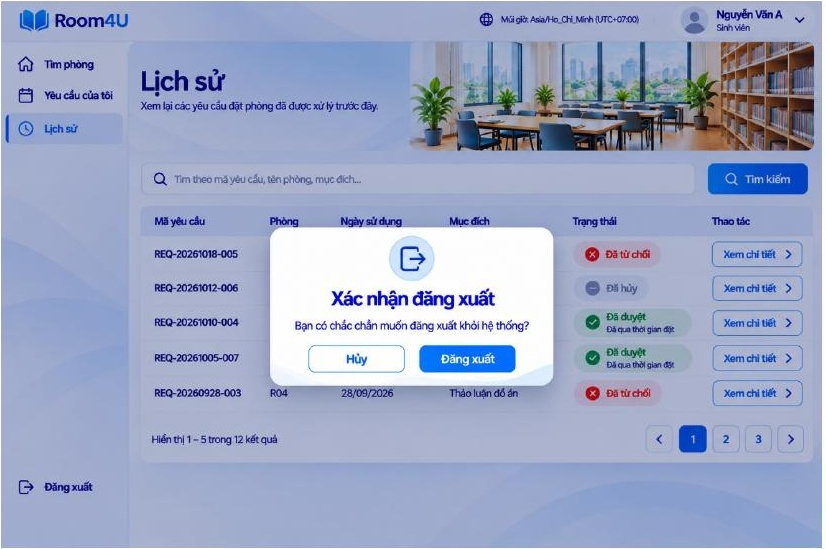
\includegraphics[width=\textwidth,height=0.72\textheight,keepaspectratio]{images/figures/image9.jpg}
\emph{\textbf{Figure 7.2.4.3.} S04 -- History page with Log Out
confirmation.}
\end{center}


\subsubsection{7.2.5. S05 -- Admin Request
Queue}\label{s05-admin-request-queue}

\textbf{Description:} This screen is the administrator's
request-management queue. It provides status categories for Pending,
Approved, Rejected, and Cancelled requests, together with a search field
and a submission-date filter. The request table displays key information
such as request ID, room, requested usage period, number of
participants, submission time, and current status. Administrators select
View Details to inspect and process an individual request.

\textbf{Interaction and Error Handling:} The queue is a read view.
Loading or filtering it does not process a request. Pending is the
default status filter. The Approved filter is required to find bookings
for UC-10. Selecting View Details opens S06. If no request matches the
filters, an empty-state message is displayed; if loading fails, the
administrator can retry.

\begin{center}
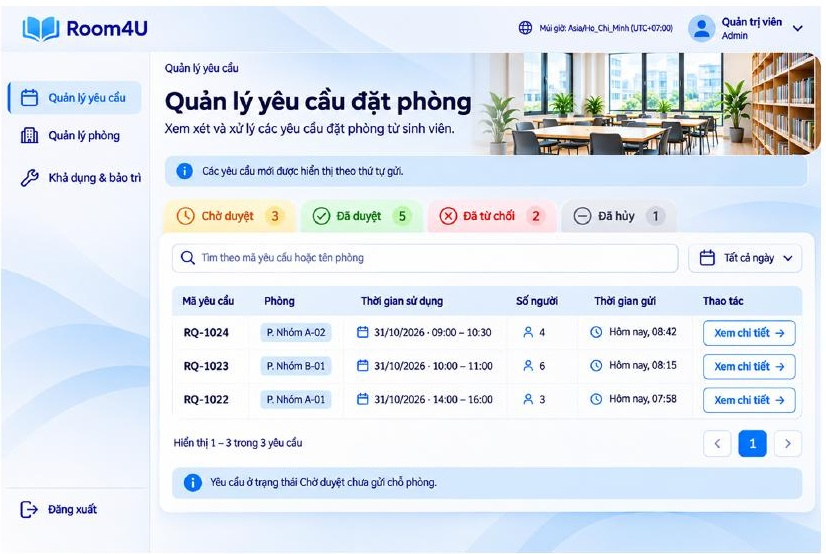
\includegraphics[width=\textwidth,height=0.72\textheight,keepaspectratio]{images/figures/image10.jpg}
\emph{\textbf{Figure 7.2.5.} S05 -- Admin Request Queue.}
\end{center}


\subsubsection{7.2.6. S06 -- Booking Request Details and
Processing}\label{s06-booking-request-details-and-processing}

\textbf{Description:} This screen presents the details and processing
controls for a selected booking request. Its layout changes according to
the request status. Common information includes booking details,
requester information, room information, the room schedule, and
request-processing history.

Pending Requests: Administrators review the requested date and time,
duration, number of participants, purpose, notes, requester details,
room capacity, equipment, and room availability. A Pending request can
be approved only if its scheduled start time has not been reached and
all current scheduling, room, and capacity checks pass. A Pending
request whose start time has arrived or passed must not be approved, but
it may still be rejected by providing a valid rejection reason. Before
approval, the system checks for scheduling conflicts. If the requested
period is no longer available, the interface displays a conflict message
and does not approve the request.

Approved, Rejected, and Cancelled Requests: Administrators can review
the booking information, current status, processing reason when
applicable, and request history. For an Approved request, the Cancel
Booking action is available only before its scheduled start time. The
administrator must enter a valid cancellation reason of 1--250
characters after leading and trailing whitespace are trimmed, and
explicitly confirm the action (BR-13). Rejected and Cancelled requests
are presented for review rather than as pending requests awaiting
approval.

\textbf{Control Specifications}

\small
\setlength{\tabcolsep}{3pt}
\renewcommand{\arraystretch}{1.15}
\begin{longtable}[]{@{}
  >{\raggedright\arraybackslash}p{0.15557200000000002\textwidth}
  >{\raggedright\arraybackslash}p{0.15557200000000002\textwidth}
  >{\raggedright\arraybackslash}p{0.317952\textwidth}
  >{\raggedright\arraybackslash}p{0.290904\textwidth}@{}}
\hline
\begin{minipage}[b]{\linewidth}\raggedright
\textbf{Control}
\end{minipage} & \begin{minipage}[b]{\linewidth}\raggedright
\textbf{Type}
\end{minipage} & \begin{minipage}[b]{\linewidth}\raggedright
\textbf{Description and Validation}
\end{minipage} & \begin{minipage}[b]{\linewidth}\raggedright
\textbf{Event Handling}
\end{minipage} \\
\hline
\endhead
\hline
\endlastfoot
\textbf{Current request details} & Read-only detail & Shows request
status, room/capacity, requester information, booking time, participant
count, and processing history. & Refresh current data before retrying an
action based on stale information. \\
\textbf{Approve} & Button + confirmation & Available only for a Pending
request whose scheduled start time has not been reached. Approval is
subject to current scheduling, room availability, and capacity checks. &
Successful approval updates status; a conflict prevents approval and
displays the cause. \\
\textbf{Reject reason} & Text area + confirmation & Required for
rejection; 1--250 characters after leading and trailing whitespace are
trimmed. A Pending request may still be rejected even when its scheduled
start time has arrived or passed. & Invalid reason is retained with
validation feedback; valid confirmation processes rejection. \\
\textbf{Cancel Booking} & Conditional button + reason & Available only
for an Approved request before its scheduled start time. A valid reason
of 1--250 characters after trimming is required, together with explicit
administrator confirmation (BR-13). & Confirmation processes
cancellation and updates the request to Cancelled. \\
\textbf{Conflict information} & Administrator information panel & Shows
the relevant conflict; does not automatically cancel or modify another
booking. & Administrator reviews the conflict and returns to the request
detail. \\
\end{longtable}
\normalsize

Error Handling: If the request is no longer Pending, approval or
rejection is not performed. A Pending request whose scheduled start time
has arrived or passed cannot be approved, but can still be rejected with
a valid reason. If the requested period conflicts with current
availability, the system displays the conflict and leaves the request
unchanged. For Approved requests, cancellation is allowed only before
the scheduled start time and requires a valid reason and explicit
confirmation. If cancellation is not permitted, the interface explains
why.

\begin{center}
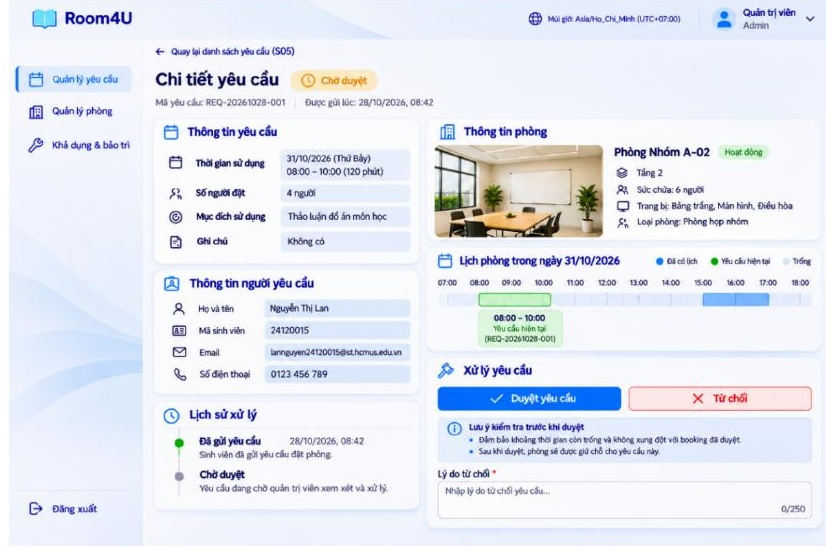
\includegraphics[width=\textwidth,height=0.72\textheight,keepaspectratio]{images/figures/image11.jpg}
\emph{\textbf{Figure 7.2.6.1.} S06.1 -- Pending Request Details.}
\end{center}


\begin{center}
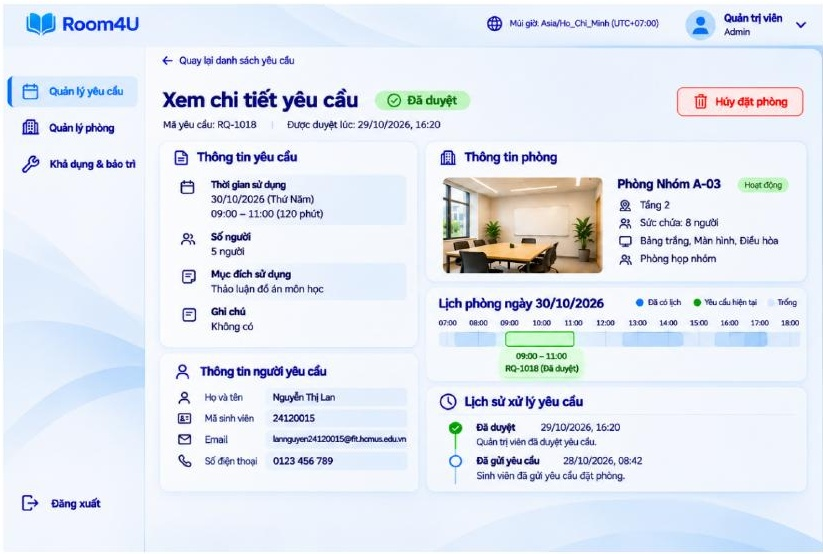
\includegraphics[width=\textwidth,height=0.72\textheight,keepaspectratio]{images/figures/image12.jpg}
\emph{\textbf{Figure 7.2.6.2.} S06.2 -- Approved Request Details and
Cancellation.}
\end{center}


\begin{center}
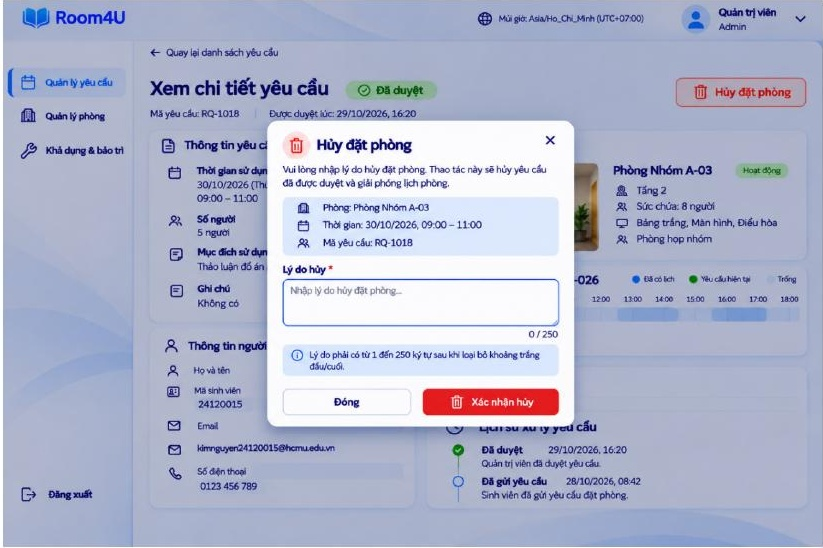
\includegraphics[width=\textwidth,height=0.72\textheight,keepaspectratio]{images/figures/image13.jpg}
\emph{\textbf{Figure 7.2.6.3.} S06.2 -- Approved Booking Cancellation
dialog.}
\end{center}


\subsubsection{7.2.7. S07 -- Room Management}\label{s07-room-management}

\textbf{Description:} This screen allows administrators to manage room
records and monitor each room's current status. It loads the room list
and summary from GET /admin/rooms. Summary cards show the total number of
rooms and mutually exclusive counts of Active, Under Maintenance, and
Suspended rooms. The API classifies every room using one server-selected
asOf: a suspended room is Suspended; an active room with an active
maintenance block satisfying startAt $\leq$ asOf $<$ endAt is Under
Maintenance; every other active room is Active. The same asOf is used
for the list and summary, and the summary always covers all rooms,
regardless of the current list filters. Administrators can search by
room code or name and filter the list by floor or display status. The
room table and detail panel show the room code, room name, floor,
capacity, equipment, description, and display status. After a successful
add, edit, suspend, or resume operation, S07 reloads both the list and
summary.

Room Creation: The Add Room dialog collects a unique room code, room
name, floor, capacity, equipment selections, an optional description, and
an optional selection of an existing room image. The room code must be unique without case sensitivity after
leading and trailing whitespace are removed. The room name is required
and must contain 1--80 characters after trimming leading and trailing
whitespace. Capacity must be an integer from 1 to 50. Equipment
selections come from the complete ADR-005 equipment catalogue, including
``Ổ cắm điện''. The frontend submits
selected equipment as an equipmentCodes array; an empty array means no
equipment is selected. The description is optional and limited to 250
characters. The selected image is submitted as photoRef; when blank, omitted
or null on creation, the default room image is used. After a valid
submission, a success dialog confirms that the new room has been added
and shows its key details.

Room Editing: The Edit Room dialog displays the selected
room's existing information for update. Administrators
can update the room code, name, floor, capacity, equipment, optional
description, and optional selection of an existing room image. The room name remains required and must contain 1--80
characters after trimming. The internal room ID remains unchanged. The
room code may be updated subject to the uniqueness rules in BR-14. When
the edit dialog opens, the frontend reads the room's
equipmentCodes from the API and preselects the matching checkboxes from
the complete ADR-005 catalogue. When saving, the frontend submits the
selected codes as an equipmentCodes array; an empty array means no
equipment is selected. Room4U revalidates the fields, including
room-code uniqueness, and checks the proposed capacity against current
future Approved bookings. When the edit dialog opens, it shows the
current photo. On update, omitting photoRef preserves the current image,
null clears the selection and uses the default image, and a valid
existing-image reference selects that image. The image-removal control
submits null. After a valid update, a success dialog confirms that the
room information has been updated.

\textbf{Suspend and Resume:} The room detail panel provides the
applicable room-status action. When a suspended room is resumed,
existing Approved bookings and maintenance schedules are preserved.
Resume restores the ability to receive new booking requests only for
time periods that remain valid; it does not cancel, modify, or overwrite
existing bookings or maintenance records.

\textbf{Control Specifications}

\small
\setlength{\tabcolsep}{3pt}
\renewcommand{\arraystretch}{1.15}
\begin{longtable}[]{@{}
  >{\raggedright\arraybackslash}p{0.15557200000000002\textwidth}
  >{\raggedright\arraybackslash}p{0.14885600000000002\textwidth}
  >{\raggedright\arraybackslash}p{0.33147600000000005\textwidth}
  >{\raggedright\arraybackslash}p{0.284096\textwidth}@{}}
\hline
\begin{minipage}[b]{\linewidth}\raggedright
\textbf{Control}
\end{minipage} & \begin{minipage}[b]{\linewidth}\raggedright
\textbf{Type}
\end{minipage} & \begin{minipage}[b]{\linewidth}\raggedright
\textbf{Description and Validation}
\end{minipage} & \begin{minipage}[b]{\linewidth}\raggedright
\textbf{Event Handling}
\end{minipage} \\
\hline
\endhead
\hline
\endlastfoot
\textbf{Room search} & Text input & Sends optional q to GET /admin/rooms; q matches room code or name without case sensitivity. & Refreshes the filtered room list and its total; summary counts remain unfiltered. \\
\textbf{Floor / status filters} & Selection controls & Sends optional floor and status values to GET /admin/rooms; status uses the API displayStatus values. & Applies filters before pagination without changing room records; keeps the all-room summary unchanged. \\
\textbf{Room details} & Read-only / editable fields & Displays room
code, name, floor, capacity, equipment, description, and status. &
Selecting a room opens its detail panel. \\
\textbf{Add / Edit Room} & Dialog + inputs & Unique case-insensitive
room code; required room name of 1--80 characters after trimming; floor;
integer capacity 1--50; equipmentCodes array from the complete ADR-005
catalogue; optional description $\leq$250 characters; optional image
reference photoRef. & Save validates fields and room-code uniqueness.
Create/update submits equipmentCodes; empty array means none. Edit
preselects equipment from the API and preserves the internal room ID.
Successful changes reload the room list and summary. \\
\textbf{Save} & Button & Checks proposed capacity against current future
Approved bookings. & Valid save updates room details; failure leaves
stored data unchanged. \\
\textbf{Suspend / Resume} & Contextual button + confirmation & Action
depends on current room status. & Updates room status under UC-12;
existing Approved bookings and maintenance schedules are preserved. \\
Equipment & Multi-select checkboxes & Uses all equipment options in
ADR-005, including Ổ cắm điện. Selected values are represented by
equipmentCodes; an empty array means no equipment is selected. &
Create/update submits the selected code array. Opening Edit Room
restores checkbox states from the API equipmentCodes. \\
\textbf{Room photo} & Optional existing-image selector & Optional image
reference submitted as photoRef. On create, blank, omitted or null uses the
default image. On update, omitted preserves the current image; null
clears it. & Edit opens with the current image; selecting a preloaded
image submits its reference, and the remove-image action submits null. \\
\end{longtable}
\normalsize

\begin{center}
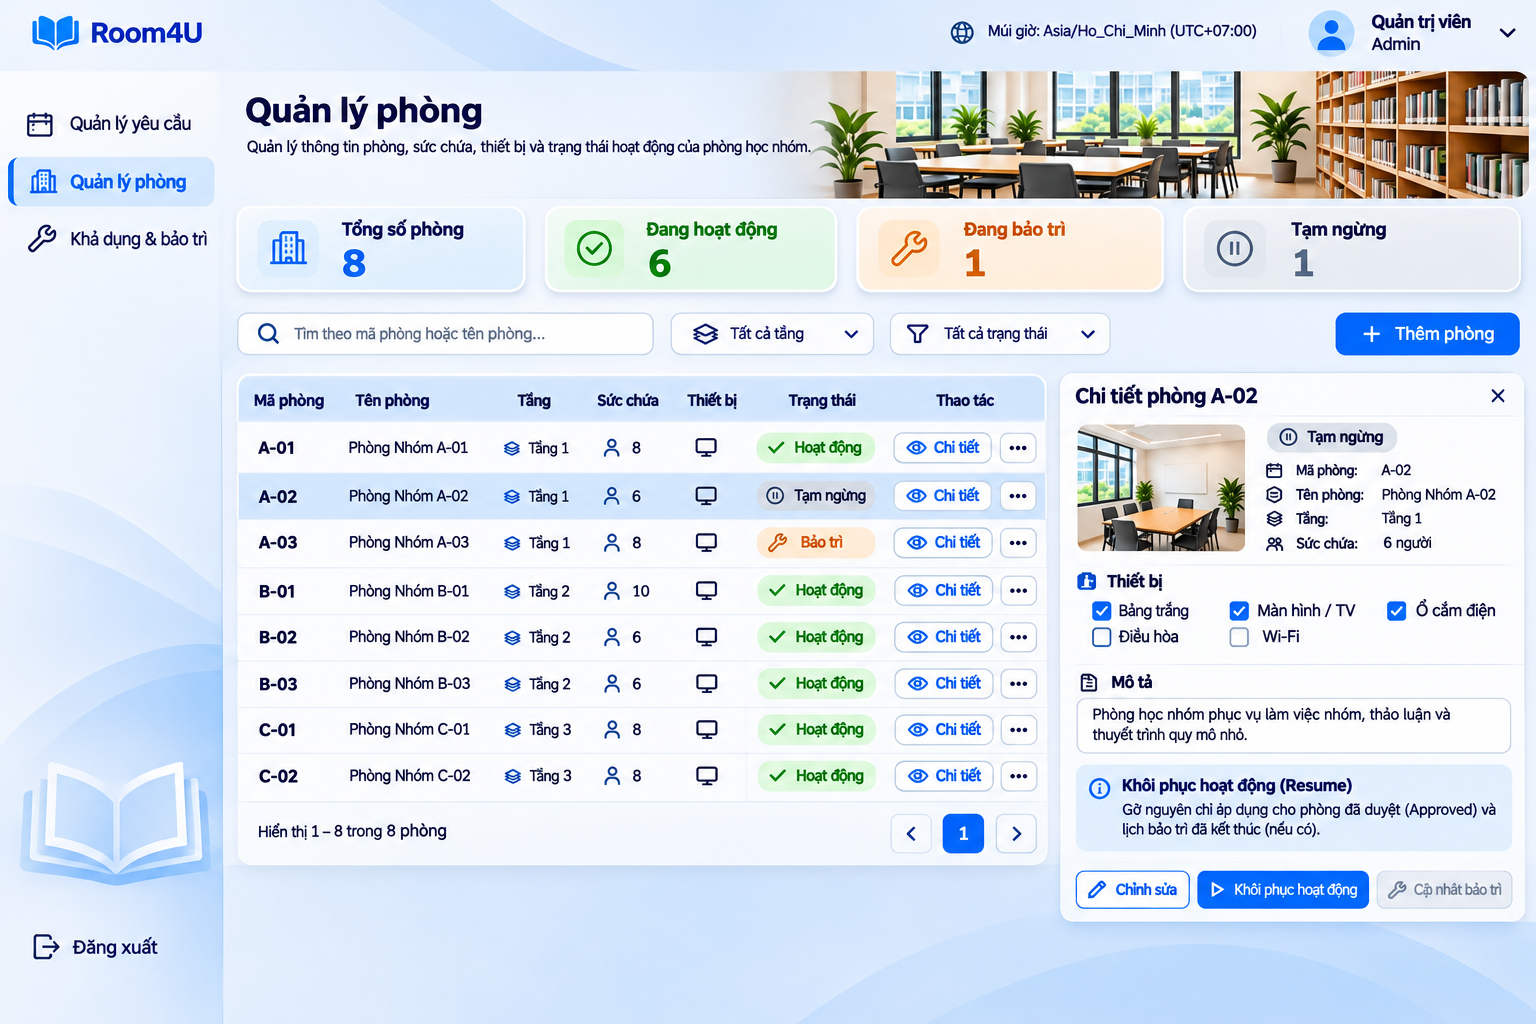
\includegraphics[width=\textwidth,height=0.72\textheight,keepaspectratio]{images/figures/image14.png}
\emph{\textbf{Figure 7.2.7.} S07 -- Room Management.}
\end{center}


\subsubsection{7.2.8. S08 -- Room Availability and
Maintenance}\label{s08-room-availability-and-maintenance}

\textbf{Description:} This screen allows administrators to inspect room
usage and manage maintenance schedules. The interface separates the
room-usage calendar from the maintenance schedule so that Approved
bookings and maintenance records can be reviewed without confusing their
meanings.

\textbf{Room Usage History:} Administrators can inspect room schedules
in the available calendar views and identify Approved bookings,
maintenance periods, and available time slots. The schedule is organized
by room and date to support availability checks.

Maintenance Schedule: Administrators can view existing maintenance
records, create a maintenance schedule, inspect its details, and remove
its effect when eligible. A maintenance record identifies the affected
room, start and end time, reason, and status. The maintenance reason is
required and must contain 1--250 characters after leading and trailing
whitespace are trimmed. The maintenance list provides view and remove
actions; an edit action is not included in the current UC-13 flow.

Maintenance Rules and Removal Flow: To create a maintenance schedule,
the administrator specifies the room, start time, end time, and reason.
The reason is mandatory and must contain 1--250 characters after
trimming leading and trailing whitespace. The end time must be later
than the start time. The system rejects creation if the requested period
overlaps an Approved booking or an active maintenance period.
Maintenance schedules are not subject to booking-specific restrictions:
the 08:00--20:00 operating window, booking-duration options, and
same-calendar-day requirement do not apply. Creating maintenance does
not automatically cancel or modify an Approved booking. To remove a
schedule's effect, the administrator selects a block
that is Active and has not started, reviews the information, and
confirms the action. On success, the system removes the
block's effect on availability, updates the room
schedule, and retains the maintenance record for reference. If the block
has already started or no longer meets the eligibility conditions, the
system displays an error and makes no change to the record.

When maintenance creation returns HTTP 409 with
error.code = SCHEDULE\_CONFLICT, S08 reads error.conflicts and retains
error.requestId as the response correlation identifier. Following SQ05,
if Approved bookings overlap, the API returns those conflicts first, each
with bookingRequestId, startAt and endAt. S08 displays the list and lets
the Administrator open each booking in S06. The Administrator may cancel
a booking only when UC-10 permits it; if it has started or is otherwise
ineligible, S08 instructs the Administrator to choose another time
window. The Administrator returns to S08 and retries after handling any
eligible booking separately. If there is no Approved-booking conflict
but an active maintenance block overlaps, S08 displays its
maintenanceBlockId and interval and instructs the Administrator to
choose another time window. No booking is cancelled automatically.

\textbf{Control Specifications}

\small
\setlength{\tabcolsep}{3pt}
\renewcommand{\arraystretch}{1.15}
\begin{longtable}[]{@{}
  >{\raggedright\arraybackslash}p{0.15557200000000002\textwidth}
  >{\raggedright\arraybackslash}p{0.14885600000000002\textwidth}
  >{\raggedright\arraybackslash}p{0.33147600000000005\textwidth}
  >{\raggedright\arraybackslash}p{0.284096\textwidth}@{}}
\hline
\begin{minipage}[b]{\linewidth}\raggedright
\textbf{Control}
\end{minipage} & \begin{minipage}[b]{\linewidth}\raggedright
\textbf{Type}
\end{minipage} & \begin{minipage}[b]{\linewidth}\raggedright
\textbf{Description and Validation}
\end{minipage} & \begin{minipage}[b]{\linewidth}\raggedright
\textbf{Event Handling}
\end{minipage} \\
\hline
\endhead
\hline
\endlastfoot
\textbf{Room usage calendar} & Calendar & Displays room schedules by
room and date; distinguishes Approved bookings, maintenance, and
available periods. & Changing room/date/view refreshes schedule
information. \\
\textbf{Maintenance interval} & Start/end date and time & End time must
be later than start time; interval is checked against Approved bookings
and active maintenance. Booking-only restrictions (08:00--20:00, booking
duration, and same-day requirement) do not apply. & Invalid interval
displays validation; conflict rejects creation. \\
\textbf{Maintenance reason} & Text area & Required text area; 1--250
characters after leading and trailing whitespace are trimmed. & A valid
reason is stored with the maintenance record; invalid or blank input is
rejected. \\
\textbf{Create maintenance} & Button + confirmation & Creates a record
only when no prohibited overlap exists. & On 409 SCHEDULE\_CONFLICT,
shows error.conflicts. Approved-booking conflicts include booking ID
and interval and link to S06; cancellation is offered only when UC-10
allows it. If a booking has started or an active maintenance block is
the conflict, instructs the Administrator to choose another time.
Successful creation updates the schedule and maintenance list. \\
\textbf{Maintenance list} & List / table & Shows affected room,
start/end time, reason, and status; supports view and eligible removal.
& Selecting a record opens its details. \\
\textbf{Remove maintenance} & Button + confirmation & Only an Active
block that has not started can be removed. & Successful removal
deactivates the block's effect but retains the record;
unsuccessful removal leaves it unchanged. \\
\end{longtable}
\normalsize

\begin{center}
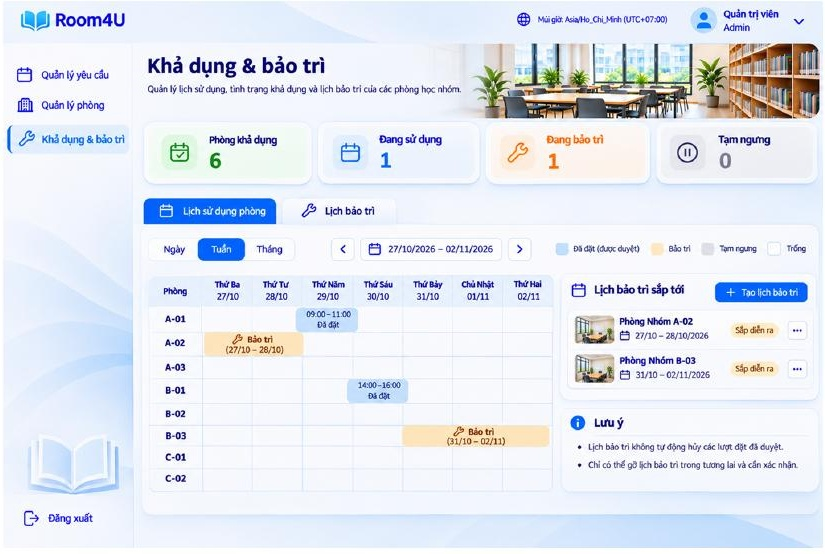
\includegraphics[width=\textwidth,height=0.72\textheight,keepaspectratio]{images/figures/image15.jpg}
\emph{\textbf{Figure 7.2.8.1.} S08.1 -- Room Usage History.}
\end{center}


\begin{center}
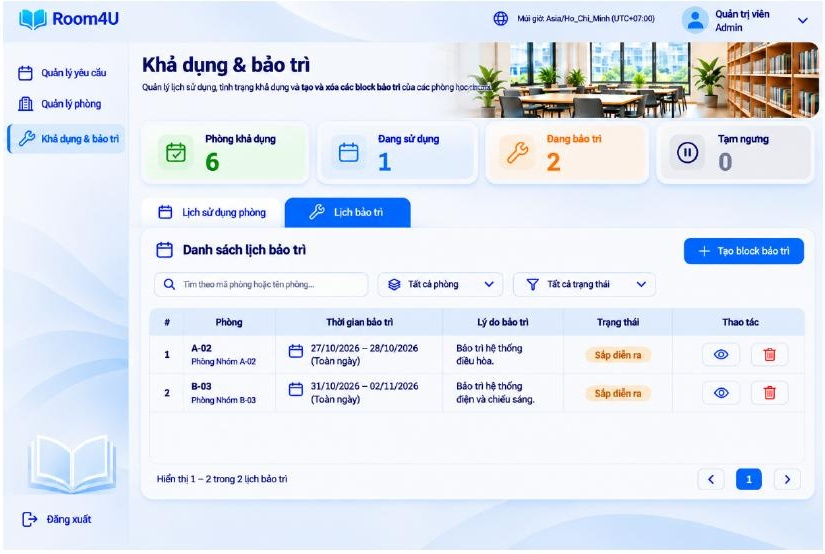
\includegraphics[width=\textwidth,height=0.72\textheight,keepaspectratio]{images/figures/image16.jpg}
\emph{\textbf{Figure 7.2.8.2.} S08.2 -- Maintenance Schedule.}
\end{center}


\subsubsection{7.2.9. UI-to-API Data Mapping}\label{ui-to-api-data-mapping}

The following mapping defines how the affected UI controls correspond to
API/database fields. Field names follow the API contract; purpose and
equipment codes follow the catalogues in ADR-005. Vietnamese labels are
presentation values and do not replace the stored codes.

\small
\setlength{\tabcolsep}{3pt}
\renewcommand{\arraystretch}{1.15}
\begin{longtable}[]{@{}
  >{\raggedright\arraybackslash}p{0.23\textwidth}
  >{\raggedright\arraybackslash}p{0.23\textwidth}
  >{\raggedright\arraybackslash}p{0.23\textwidth}
  >{\raggedright\arraybackslash}p{0.23\textwidth}@{}}
\hline
\begin{minipage}[b]{\linewidth}\raggedright
\textbf{Screen}
\end{minipage} & \begin{minipage}[b]{\linewidth}\raggedright
\textbf{UI control}
\end{minipage} & \begin{minipage}[b]{\linewidth}\raggedright
\textbf{API/database field}
\end{minipage} & \begin{minipage}[b]{\linewidth}\raggedright
\textbf{Data handling}
\end{minipage} \\
\hline
\endhead
\hline
\endlastfoot
S02 & Equipment filters & equipmentCodes & Optional array of equipment
codes (catalogue in ADR-005). Multiple selections use AND logic; an
empty selection applies no equipment filter. \\
S03 & Purpose of use & purpose & Required string purpose code from ADR-005;
submit the code, display its Vietnamese label, and store it in
booking\_requests.purpose. \\
S03 & Optional note & note & Optional string, maximum 250 characters; trim input and normalize blank to NULL. \\
S03 & Submission retry & submissionKey & Required UUID key for one
logical submission; reuse it only when retrying the same unchanged
submission after timeout or uncertain response. \\
S04 & Purpose display & purpose & Read the code from the purpose field
returned by the API (stored in booking\_requests.purpose) and resolve it
to the corresponding Vietnamese display label. \\
S04 & Mô tả chi tiết yêu cầu & note & Display the note value; this is
not a separate field. \\
S07 & Equipment checkboxes & equipmentCodes & Array of codes from ADR-005; required on create, optional on update (omitted means preserve), and an empty array means none selected. Edit Room restores values from API equipmentCodes. \\
S07 & Room list and summary & items, total, summary, asOf,
displayStatus & GET /admin/rooms returns the filtered page and total plus
an all-room summary. One server asOf classifies the list and summary;
suspended takes precedence over active maintenance, then active. \\
S07 & Search and filters & q, floor, status, page, pageSize & Optional
query and pagination inputs to GET /admin/rooms; q matches room code/name
case-insensitively. Filter before pagination and sort by code then ID. \\
S07 & Optional room image & photoRef & Create: blank, omitted or null uses the
default. Update: omission preserves, null clears, and a valid existing
image reference selects. The remove-image action sends null. \\
\end{longtable}
\normalsize

\subsection{Responsive Layout and
Accessibility}\label{responsive-layout-and-accessibility}

\subsubsection{7.3.1. Responsive Layout}\label{responsive-layout}

Room4U uses a desktop-first layout while adapting its interface to
smaller mobile screens. The same business rules and available operations
are retained; only the presentation and arrangement of controls change.

\small
\setlength{\tabcolsep}{3pt}
\renewcommand{\arraystretch}{1.15}
\begin{longtable}[]{@{}
  >{\raggedright\arraybackslash}p{0.169096\textwidth}
  >{\raggedright\arraybackslash}p{0.372048\textwidth}
  >{\raggedright\arraybackslash}p{0.378856\textwidth}@{}}
\hline
\begin{minipage}[b]{\linewidth}\raggedright
\textbf{Interface Element}
\end{minipage} & \begin{minipage}[b]{\linewidth}\raggedright
\textbf{Desktop Layout}
\end{minipage} & \begin{minipage}[b]{\linewidth}\raggedright
\textbf{Mobile Layout}
\end{minipage} \\
\hline
\endhead
\hline
\endlastfoot
\textbf{Header} & Room4U branding, account information, and navigation
controls. & Compact header to preserve screen space. \\
\textbf{Sidebar} & Vertical navigation items. & Compact or collapsible
navigation. \\
\textbf{Room cards} & Multiple room cards in a grid. & Cards stacked
vertically. \\
\textbf{Booking form} & Structured form layout with grouped fields. &
Fields stacked vertically without changing duration-based booking
input. \\
\textbf{Request tables} & Tabular request information. & Compact cards
or responsive list to avoid page-level horizontal scrolling. \\
\textbf{Availability calendar} & Schedule with space for time-slot
information. & Simplified or horizontally manageable schedule. \\
\textbf{Dialogs} & Confirmation and result dialogs over the current
screen. & Dialog width adapts to viewport while keeping actions
readable. \\
\end{longtable}
\normalsize

Proposed verification viewport sizes are Desktop 1366 × 768 pixels and
Mobile 390 × 844 pixels. The layout should avoid fixed-width page
containers that cause horizontal scrolling. The PA2 mockups provide the
desktop visual baseline; the PA3 mobile layout is a responsive proposal
and must be verified during implementation.

\subsubsection{7.3.2. Accessibility
Considerations}\label{accessibility-considerations}

\small
\setlength{\tabcolsep}{3pt}
\renewcommand{\arraystretch}{1.15}
\begin{longtable}[]{@{}
  >{\raggedright\arraybackslash}p{0.16238\textwidth}
  >{\raggedright\arraybackslash}p{0.39909600000000006\textwidth}
  >{\raggedright\arraybackslash}p{0.358524\textwidth}@{}}
\hline
\begin{minipage}[b]{\linewidth}\raggedright
\textbf{Checklist Item}
\end{minipage} & \begin{minipage}[b]{\linewidth}\raggedright
\textbf{Proposed Implementation}
\end{minipage} & \begin{minipage}[b]{\linewidth}\raggedright
\textbf{Verification Required}
\end{minipage} \\
\hline
\endhead
\hline
\endlastfoot
\textbf{Contrast and meaning} & Text contrast ≥4.5:1; status meaning is
conveyed by text labels, not color alone. & Measure actual implemented
colors; do not claim compliance from wireframes. \\
\textbf{Keyboard access} & Native buttons/links, logical tab order,
visible focus, and dialog focus restoration. & Walk through sign-in,
search, submit, cancel, and approve. \\
\textbf{Labels and errors} & Persistent labels; field-error
associations; status region; preserve safe values. & Verify announced
errors, confirmation dismissal, and retry behavior. \\
\textbf{Responsive layout} & Stack cards/forms; avoid fixed-width page;
mobile list cards instead of wide tables. & Test Chrome/Edge at 390×844
and 1366×768; no horizontal page scroll. \\
\textbf{Usability} & Show that Pending is not confirmed; display
room/capacity/time context. & Run the actual PA2 four-evaluator task; do
not invent participant outcomes. \\
\textbf{Localization} & Vietnamese labels and reason/error messages;
visible Asia/Ho\_Chi\_Minh time zone. & Review S01--S08 strings and
date/time conversions. \\
\end{longtable}
\normalsize

\subsubsection{7.3.3. User Feedback and Error
Communication}\label{user-feedback-and-error-communication}

\begin{itemize}
\item
  Display success feedback only after the system confirms that an
  operation has completed.
\item
  Identify missing or invalid input and explain how the user can correct
  it.
\item
  Explain scheduling conflicts and show relevant current information
  without modifying conflicting records automatically.
\item
  Use confirmation dialogs for important operations, including booking
  submission, cancellation, approval, rejection, room
  suspension/resumption, and maintenance removal where applicable.
\item
  Preserve valid input after known validation or conflict failures so
  users can correct the request.
\item
  Clearly distinguish Pending from Approved; a Pending request is
  awaiting administrator review and is not a confirmed reservation.
\end{itemize}

\subsubsection{7.3.4. Usability and
Localization}\label{usability-and-localization}

The interface should show sufficient context for users to make correct
decisions. Before submitting a booking request, students should be able
to review the selected room, room capacity, usage date, start time,
duration, and calculated end time. Before administrative actions,
administrators should be able to inspect the current request or room
state.

The interface uses Vietnamese labels and messages to maintain
consistency with the target users and NFR-12. Dates and times use the
Asia/Ho\_Chi\_Minh time zone where applicable.

The usability evaluation should verify that users can complete the
following main tasks:

\begin{enumerate}
\def\labelenumi{\arabic{enumi}.}
\item
  Sign in using a provided account.
\item
  Search for a suitable meeting room.
\item
  Inspect room availability.
\item
  Submit a booking request.
\item
  Review request status and history.
\item
  Cancel an eligible booking request.
\item
  Process a booking request as an administrator.
\item
  Manage room information and maintenance schedules.
\end{enumerate}

The evaluation must follow the actual PA2 evaluation procedure and
record real observations. No participant outcomes or usability results
are assumed in this design document.
